\documentclass[tikz,border=3pt]{standalone}
\usepackage[T1]{fontenc}
\usepackage{mathptmx}
\usepackage{tikz}
\usetikzlibrary{arrows.meta,positioning,calc,fit,shapes.geometric}
\definecolor{forest}{HTML}{346E57}
\definecolor{sage}{HTML}{E8EFEA}
\definecolor{clay}{HTML}{AC653F}
\definecolor{sand}{HTML}{F4EAE2}
\definecolor{ink}{HTML}{252525}
\definecolor{gridgray}{HTML}{D8DAD6}
\tikzset{box/.style={draw=ink!65,line width=.5pt,rectangle,fill=white,align=center,font=\fontsize{10}{11.3}\selectfont,inner sep=5pt}, flow/.style={-{Latex[length=2.1mm]},line width=.65pt,draw=ink!80}, lab/.style={font=\fontsize{10}{11}\selectfont,fill=white,inner sep=2pt,align=center}}
\hyphenpenalty=10000\exhyphenpenalty=10000
\begin{document}
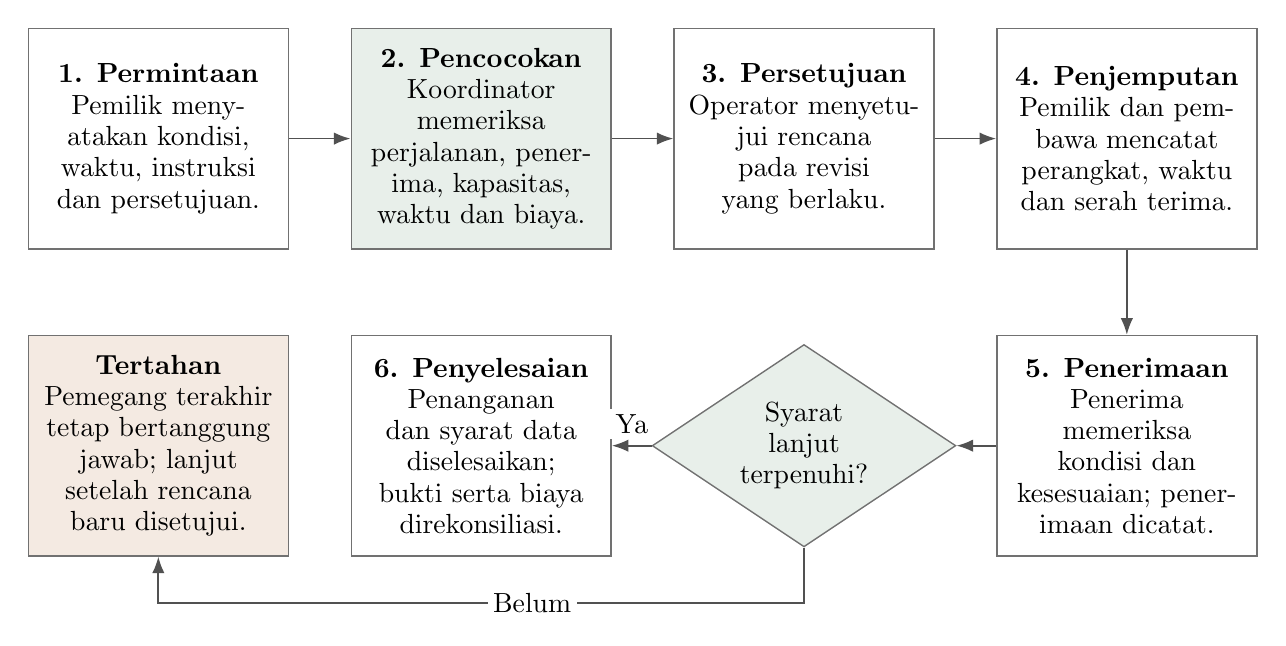
\begin{tikzpicture}[x=1cm,y=1cm]
\node[box,text width=2.95cm,minimum height=2.8cm] (s1) at (1.65,3.9) {\textbf{1. Permintaan}\\Pemilik menyatakan kondisi, waktu, instruksi dan persetujuan.};
\node[box,text width=2.95cm,minimum height=2.8cm,fill=sage] (s2) at (5.75,3.9) {\textbf{2. Pencocokan}\\Koordinator memeriksa perjalanan, penerima, kapasitas, waktu dan biaya.};
\node[box,text width=2.95cm,minimum height=2.8cm] (s3) at (9.85,3.9) {\textbf{3. Persetujuan}\\Operator menyetujui rencana pada revisi yang berlaku.};
\node[box,text width=2.95cm,minimum height=2.8cm] (s4) at (13.95,3.9) {\textbf{4. Penjemputan}\\Pemilik dan pembawa mencatat perangkat, waktu dan serah terima.};
\node[box,text width=2.95cm,minimum height=2.8cm] (s5) at (13.95,0) {\textbf{5. Penerimaan}\\Penerima memeriksa kondisi dan kesesuaian; penerimaan dicatat.};
\node[diamond,aspect=1.5,draw=ink!65,line width=.5pt,fill=sage,text width=1.85cm,align=center,inner sep=2pt,font=\fontsize{10}{11.3}\selectfont] (gate) at (9.85,0) {Syarat lanjut terpenuhi?};
\node[box,text width=2.95cm,minimum height=2.8cm] (s6) at (5.75,0) {\textbf{6. Penyelesaian}\\Penanganan dan syarat data diselesaikan; bukti serta biaya direkonsiliasi.};
\node[box,text width=2.95cm,minimum height=2.8cm,fill=sand] (hold) at (1.65,0) {\textbf{Tertahan}\\Pemegang terakhir tetap bertanggung jawab; lanjut setelah rencana baru disetujui.};
\draw[flow](s1)--(s2);\draw[flow](s2)--(s3);\draw[flow](s3)--(s4);
\draw[flow](s4.south)--(s5.north);
\draw[flow](s5.west)--(gate.east);
\draw[flow](gate.west)--node[lab,above=2pt]{Ya}(s6.east);
\draw[flow](gate.south)--++(0,-.7)-|node[lab,near start,right=2pt]{Belum}(hold.south);
\end{tikzpicture}
\end{document}
